
\documentclass[a4paper,11pt]{article}

\usepackage[utf8]{inputenc}
\usepackage{mathpazo}
\usepackage{gensymb}
\usepackage{graphicx}
\usepackage{url}
\usepackage[frenchb]{babel}
\usepackage{subfig}
\usepackage{apacite}
\usepackage{array}
\usepackage{multirow}
\usepackage{dcolumn}
\newcolumntype{d}[1]{D{,}{,}{#1}}
\usepackage[T1]{fontenc}
\usepackage{amsmath}
% \renewcommand{\thefootnote}{\Alph{footnote}}
% \usepackage[bottom]{footmisc}
% \usepackage{natbib}
% \bibliographystyle{plainnat}
% \newcommand*{\dl}{\cline{2-2}\cline{4-4}}
% \usepackage [nottoc]{tocbibind}

\begin{document}

\title{Sorgho \& Niébé au Burkina Faso}
\author{Marilyne Aza-Gnandji}
\date{\today}

\maketitle
\tableofcontents

\section{Productions agricoles au Burkina Faso}

Le Burkina Faso est un pays à économie agraire
\cite{Koulibi_FideleZONGO} d'une superficie de
274\,200\,km\textsuperscript{2} et peuplé d'environ 20 millions
d'habitants
aujourd'hui\footnote{\url{https://www.cia.gov/library/publications/the-world-factbook/geos/uv.html}}. En
2012, le secteur agro-sylvo-pastoral représente 35\,\% du PIB
burkinabé et emploie 82\,\% de la population active. Celle-ci se
répartie sur 5,7 millions d'hectares cultivés, à comparer aux 11,8
millions d'hectares de terres cultivables du Burkina
Faso\footnote{\url{http://agriculture.gouv.fr/burkina-faso}}. Aussi
l'arboriculture et le maraîchage occupent une place non négligeable
avec environ 600\,000 petites exploitations agricoles indépendantes de
moins d'un
hectare\footnote{https://www.insee.fr/fr/metadonnees/definition/c1186}.

La production agricole s'articule essentiellement autour des cultures
pluviales, notamment céréalières. Les principales cultures céréalières
sont le mil, le sorgho, le maïs et le riz. À côté de ces cultures, on
retrouve les cultures vivrières (niébé) et les cultures de rente
(coton, arachide et sésame). Les populations s'adonnent également aux
cultures de contre-saison, principalement des cultures
maraîchères\footnote{\url{https://www.mdh-limoges.org/spip.php?article2273}}.
En 2016, la production céréalière était de 4\,567\,066 tonnes soit
près de 68\,\% de la production agricole et ce pour des superficies
semées en céréales qui s'évaluaient à 4\,017\,586\,ha. Ces superficies
céréalières sont en hausse par rapport à la campagne de
2015\footnote{\url{www.insd.bf/n/contenu/pub_periodiques/tableaux_de_bord/TBE/TBE_BF_2017T1.pdf}}. L'activité
agricole au Burkina Faso est menée dans des conditions parfois
défavorables (mauvaise pluviométrie, pauvreté des sols, \ldots{}). Ce
faisant, la production agricole est faible et ne parvient pas à
couvrir les besoins alimentaires des populations.

Le Burkina Faso possède un climat tropical de type soudano-sahélien
(caractérisé par des variations pluviométriques considérables allant
d'une moyenne annuelle de 350 mm au Nord à plus de 1\,000 mm au
Sud-Ouest) avec deux saisons très contrastées : la saison des pluies
avec des précipitations comprises entre 300\,mm et 1\,200 mm et la
saison sèche durant laquelle souffle l'harmattan, un vent chaud, sec
et chargé de poussière, originaire du Sahara. La saison des pluies
dure environ 4 mois, entre mai-juin et septembre, sa durée est plus
courte au nord du
pays\footnote{http://www.burkina-faso.ca/climat-du-burkina-faso/}. Le
taux de croissance de la production agricole est de l'ordre de 4,3\,\%
pour la période 1983--2007 et, selon \citeA{Ngaido_2006}, ce taux
devrait être de 6,8\,\% pour atteindre des Objectifs du Millénaire
pour le Développement en matière de réduction de la faim. Ainsi, près
de 46\,\% de la population totale est exposé à l'insécurité
alimentaire et on estimait en 2003 le niveau de couverture des besoins
nutritionnels à 2\,283 kilocalories par personne et par jour contre
les 2\,500 kcal requis. Parallèlement, la pauvreté au Burkina est
essentiellement rurale (la contribution du milieu rural à la pauvreté
s'élevait à 92,2\,\% en 2003) et la population rurale est en grande
majorité agricole \cite{DPSAA_2011}. Le Burkina Faso a besoin d'une
croissance soutenue de sa production agricole non seulement pour
assurer sa sécurité alimentaire mais aussi pour lutter contre la
pauvreté et assurer son développement économique
\cite{Koulibi_FideleZONGO}.

\section{Le Sorgho: \emph{Sorghum bicolor} (L.) Moench}

% c\'{e}r\'{e}ales
%% Insérer dans un texte une référence de figure : (Fig.~\ref{images:photo_plante_sorgho})


% \begin{figure}[htbp]
%   \begin{center}
%     \leavevmode
%     \subfloat[Plante du Sorgho]{%
%     \label{fig-Plante du Sorgho}
%     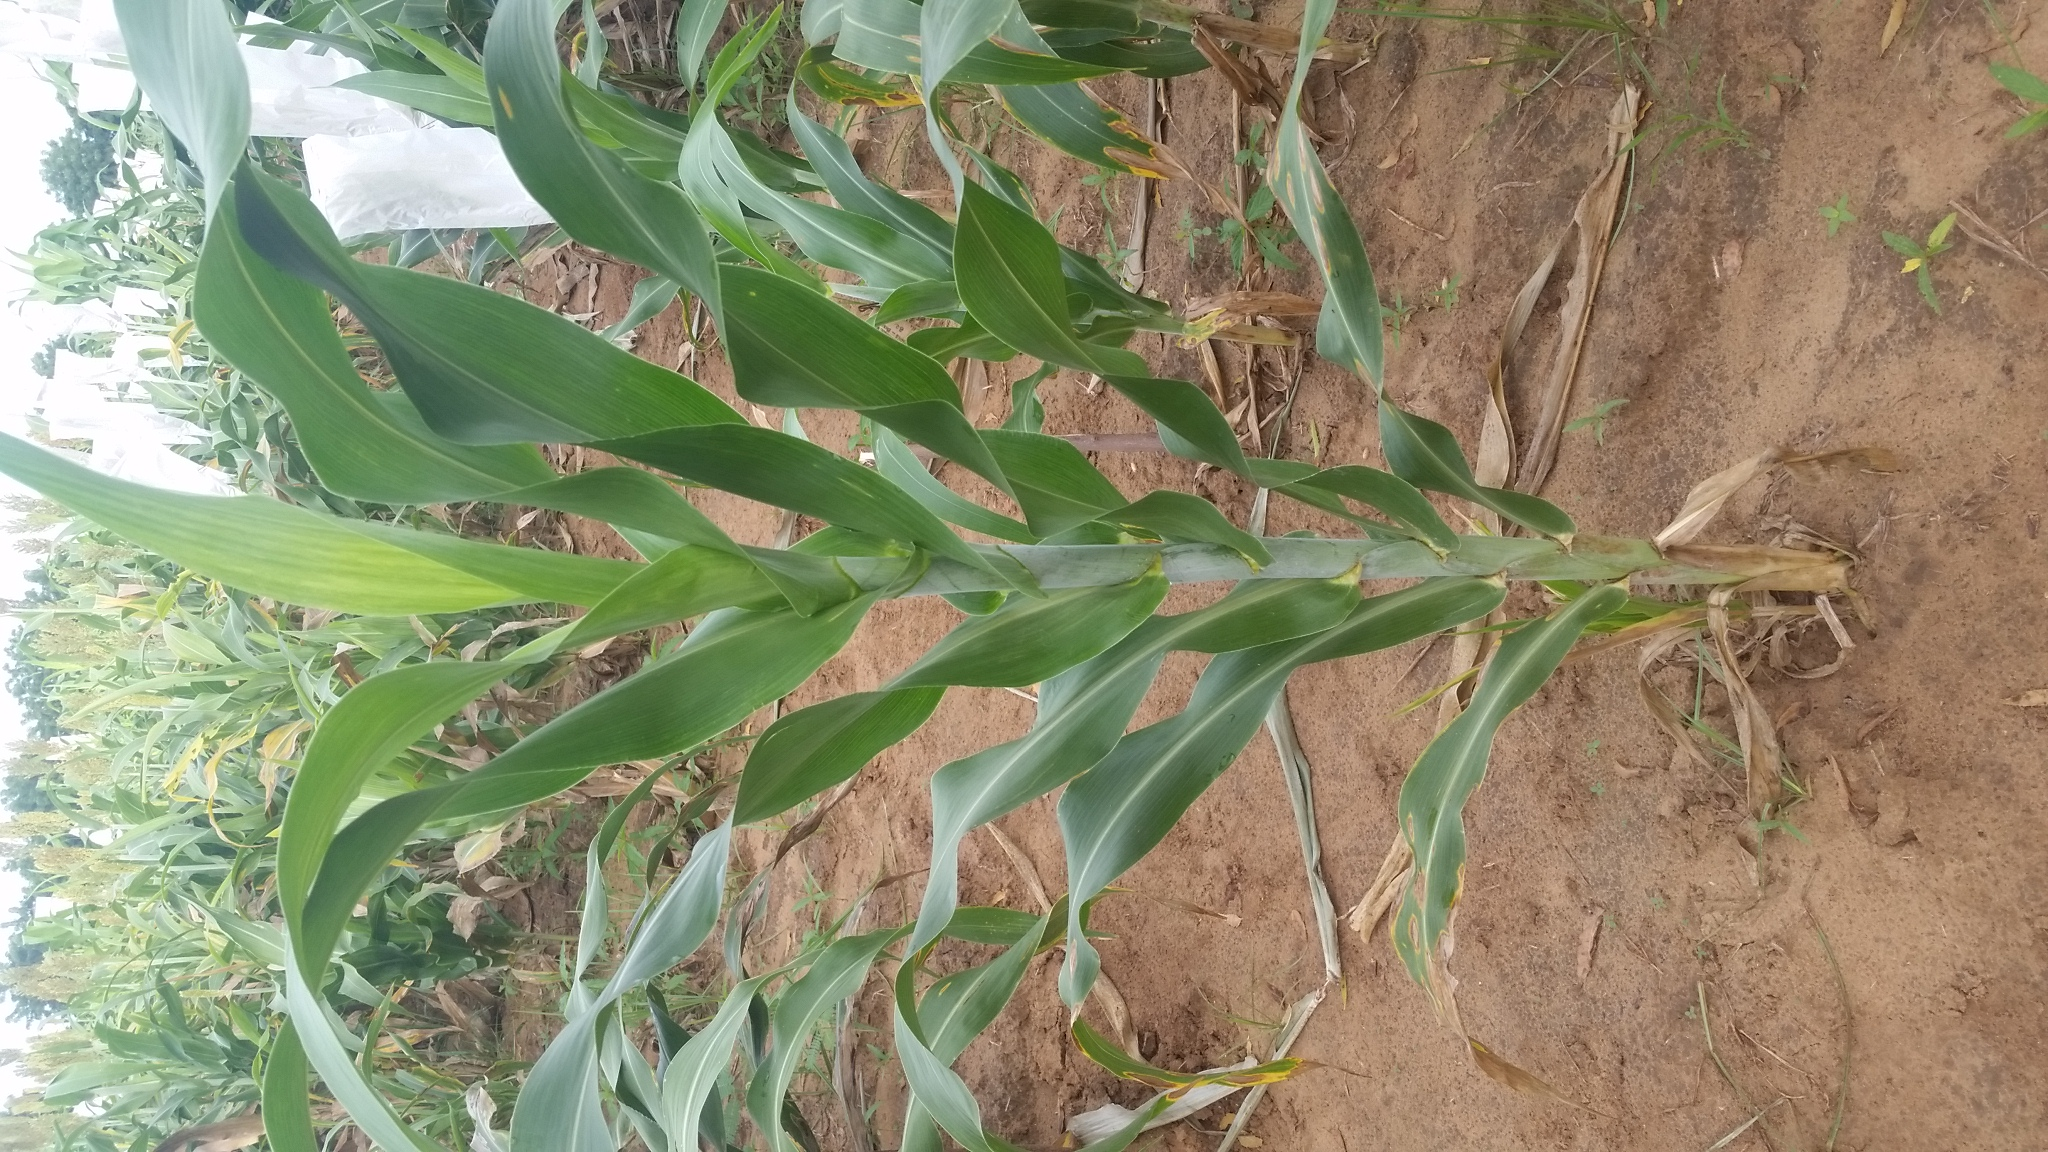
\includegraphics[width=8cm,angle=270]{images/Plante_Sorgho}}
%     \hspace{0.5cm}
%     \subfloat[Graines du Sorgho]{%
%     \label{fig-Graines du Sorgho}
%     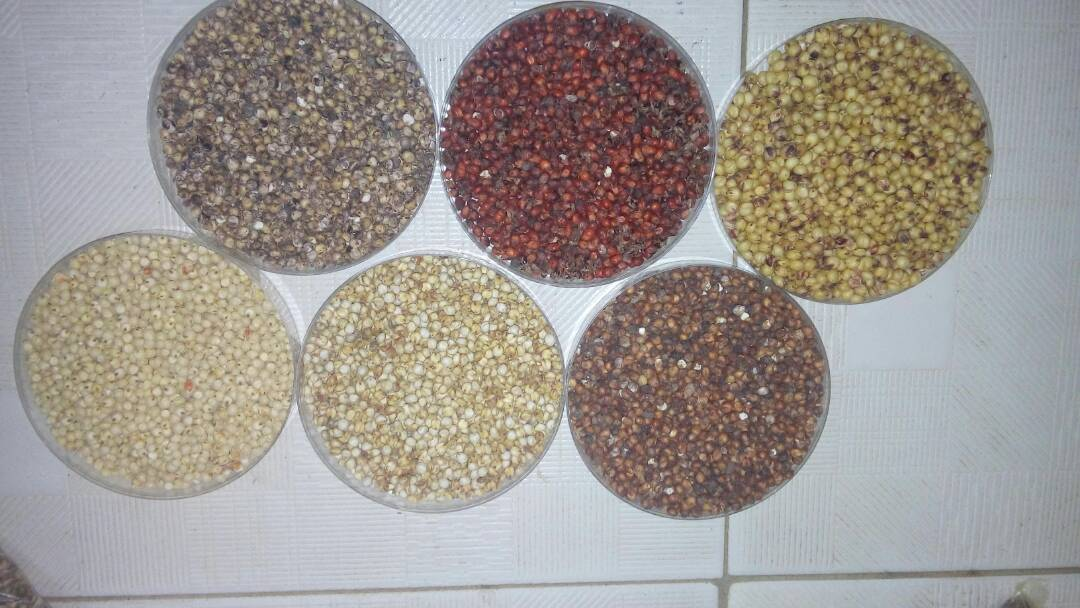
\includegraphics[width=8cm,angle=270]{images/GrainesDeSorgho}}
%     \caption{Plante,graines du sorgho-Schéma plant de sorgho et sa représentation en champ réel}
%   \end{center}
% \end{figure}



\subsection{Origine \& Diffusion}

Le sorgho est originaire de l'ancien monde et problablement de la
partie nord-est de l'Afrique où la variabilité des sorghos cultivés et
sauvages est maximale. \emph{Sorghum bicolor} (Linn.) Moench passe
généralement pour être l'appelation spécifique la plus juste pour les
sorghos cultivés \cite{food1977introduction}. Le sorgho commun
\emph{Sorghum bicolor} est une graminée très répandue à l'état sauvage
sous les climats tropicaux et subtropicaux. C'est une plante herbacée
de climat chaud qui est cultivée pour ses graines et son fourrage. Il
ressemble un peu au maïs mais son système racinaire le rend résistant
à la sécheresse ce qui fait qu'il est principalement cultivé en
Afrique pour nourrir le bétail (sorgho fourrager) et pour
l'alimentation humaine (sorgho grain). Toutefois, on le trouve aussi
beaucoup en Inde et en Amérique du Sud, ce qui le classe au 5\ieme{}
rang des céréales produites dans le monde, après le maïs, le riz, le
blé et l'orge. Selon les continents, il porte différents noms :
\og{}gros mil\fg{} en Afrique, \og{}millet indien\fg{} en Asie,
\og{}blé égyptien\fg{} au
Moyen-Orient\footnote{\url{https://jardinage.lemonde.fr/dossier-820-sorgho-sorghum-bicolor-cereale-sans-gluten.html}}. Depuis
des siècles, les peuples d'Afrique et d'Asie utilisent ses graines
pour leur alimentation. Aujourd'hui, le sorgho est cultivé sur tous
les continents, sa domestication a vraisemblablement eu lieu il y a
plusieurs millénaires en Afrique et au Sud-Est du Sahara. On note en
Afrique trois centres géographiques actifs dans la diversification du
sorgho cultivé : le centre ouest-africain qui a contribué à
l'établissement des sorghos de race guinea ; le centre est-africain
riche en sorgho des races caudatum et durra ; le centre sud-africain à
l'origine des sorghos de race kafir. Dès le troisième millénaire avant
J.-C., ces sorghos auraient gagné l'Asie : l'Inde et le Pakistan,
3\,000 ans avant J.-C., puis la Chine, un millénaire plus
tard. L'arrivée du sorgho en Europe se situerait vers 2\,000 ans avant
J.-C. Transporté en Amérique à l'époque des grandes découvertes au
\textsc{XV}\ieme{} siècle, le sorgho n'est véritablement diffusé qu'à
partir du \textsc{XIX}\ieme{} siècle, notamment aux
États-Unis\footnote{\url{https://www.gnis-pedagogie.org/sorgho-intro-caracteristiques-plante.html}}.

\subsection{Taxonomie}

Le sorgho, \emph{Sorghum bicolor (L.) Moench}, est une herbacée
annuelle de la famille des Poacées (ex-Graminées), de la sous famille
des Panicoïdeae, de la tribu des Andropogoneae et du genre
\emph{Sorghum} \cite{Doggett_1988}. C'est une espèce monoïque
préférentiellement autogame. Le taux d'allogamie varie selon la race
considérée : très faible pour les variétés cléistogames qui subissent
une autopollinisation automatique et dont les fleurs ne s'ouvrent
qu'après l'anthèse (période terminale du développement de la fleur
depuis son épanouissement jusqu'au flétrissement). Ce taux
d'autopollinisation est de l'ordre de 5 à 7\,\% pour les variétés à
panicules compactes \cite{Doggett_1988}, et varie largement (20 à
29\,\%) pour les variétés à panicules lâches de la race botanique
Guinea \cite{Ollitrault_1987,Chantereau_1994}. En champ réel les
plants de sorgho se présentent ainsi (voir
Fig.~\ref{fig-SchemaComposePage5}
p.~\pageref{fig-SchemaComposePage5}).

%% Figure 1 : schéma et représentation en champ réel d'un plant de sorgho
\begin{figure}
  \begin{center}
    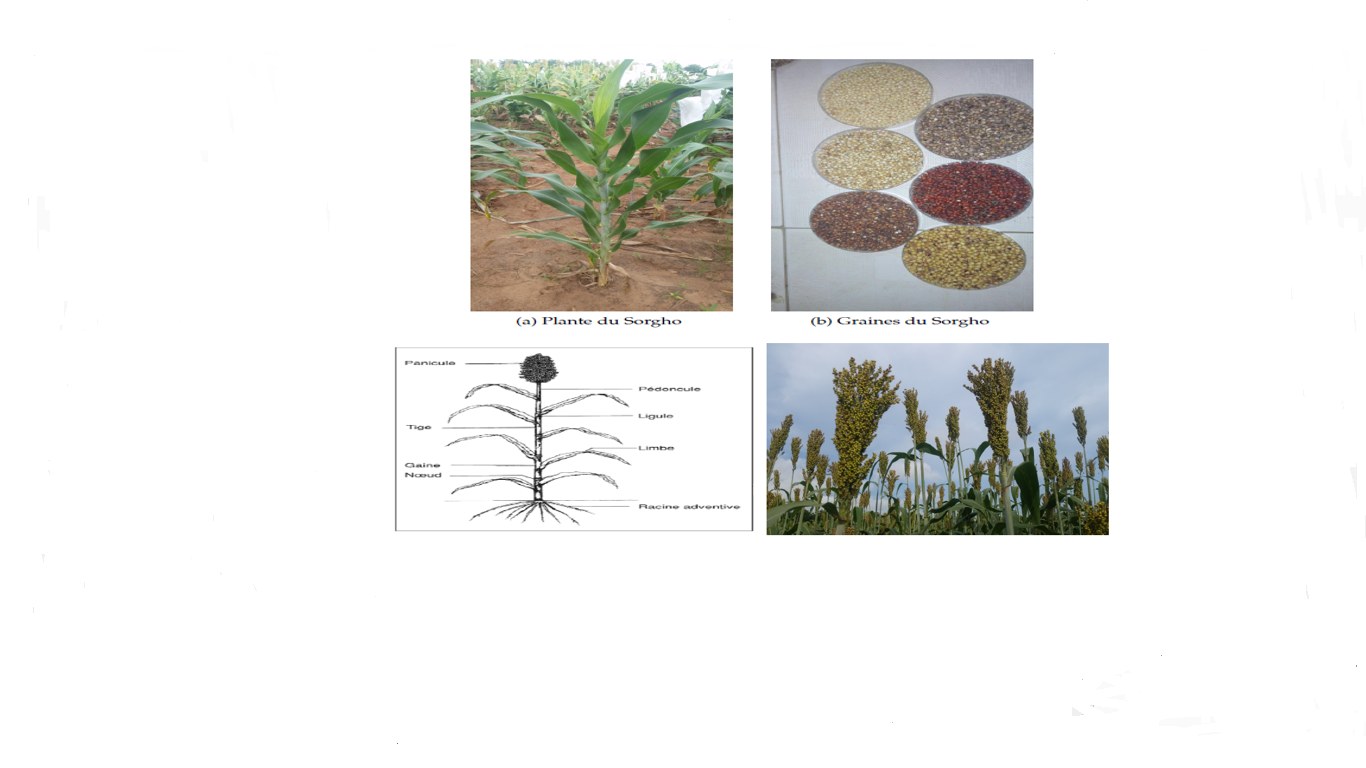
\includegraphics[width=16cm]{images/SchemaComposePage5}
  \end{center}
  \caption{Plante, graines --- Schéma et représentation en champ réel d'un plant de sorgho.}
  \label{fig-SchemaComposePage5}
\end{figure}

Par ailleurs, \citeA[p.~18]{Chantereau_2013}, résument les différentes
races du sorgho et leurs caractéristiques d'identification
(Tableau~\ref{tableau:Chantereau_2013}).

%% Tableau 1 : Principaux caractères identitaires des races du sorgho.
\begin{table}
  \begin{footnotesize}
    \begin{center}
      \begin{tabular}{lb{3cm}b{3cm}b{3cm}}
        \textbf{Race} & \textbf{Glumes}  & \textbf{Grains}  & \textbf{Panicules} \\ \hline
        Bicolor & Glumes longues recouvrant les 3/4 ou la totalité du grain  & Poids de 1000 grains de 15 à 25 g & Panicules lâches \\ \hline
        Guinea & Glumes généralement longues, ouvertes & Grains elliptiques, plus ou moins aplatis dorso-ventralement, de taille variable & Panicules lâches à semi-lâches, souvent longues à port retombant \\ \hline
        Caudatum & Glumes courtes adhérant au grain en le recouvrant partiellement & Grains dissymétriques de taille moyenne à grosse & Panicules compactes à semi-compactes souvent portées par un pédoncule crossé \\ \hline
        Durra & Glumes courtes adhérant au grain en le recouvrant partiellement & Grains plus ou moins sphériques, de taille variable mais le plus souvent gros à très gros & Panicules compactes à semi-compactes souvent portées par un pédoncule crossé \\ \hline
        Kafir & Glumes courtes adhérant au grain en le recouvrant partiellement & Grains elliptiques, de taille moyenne, poids de 1\,000 grains de 20 à 35 g & Panicules moyennement compactes, souvent de forme longue et cylindrique \\ 
      \end{tabular}
      \caption{Principaux caractères identitaires des races du sorgho \protect\cite{Chantereau_2013}.}
      \label{tableau:Chantereau_2013}
    \end{center}
  \end{footnotesize}
\end{table}

L'inflorescence est une panicule de forme variable. Le grain est un
caryopse de couleur variable (blanche, rouge, brune et jaune), qui, à
maturité, est plus ou moins dégagé des glumes
\cite{SaintClair_1989,Chantereau_1991}. Tout comme le maïs et la canne
à sucre, le sorgho appartient à la tribu des Andropogoneae. Les
Andropogoneae sont en effet, une tribu de plantes monocotylédones de
la famille des Poaceae et de la sous-famille des Panicoïdeae. La
figure~\ref{fig:phylogenie_poacees}
p.~\pageref{fig:phylogenie_poacees} illustre la classification
(cladogramme) phylogénétique des Poaceae dont fait partie le sorgho
\cite{Paquet_2005}.

%% Figure 2 : phylogénie des poacées
\begin{figure}%
  \begin{center}
    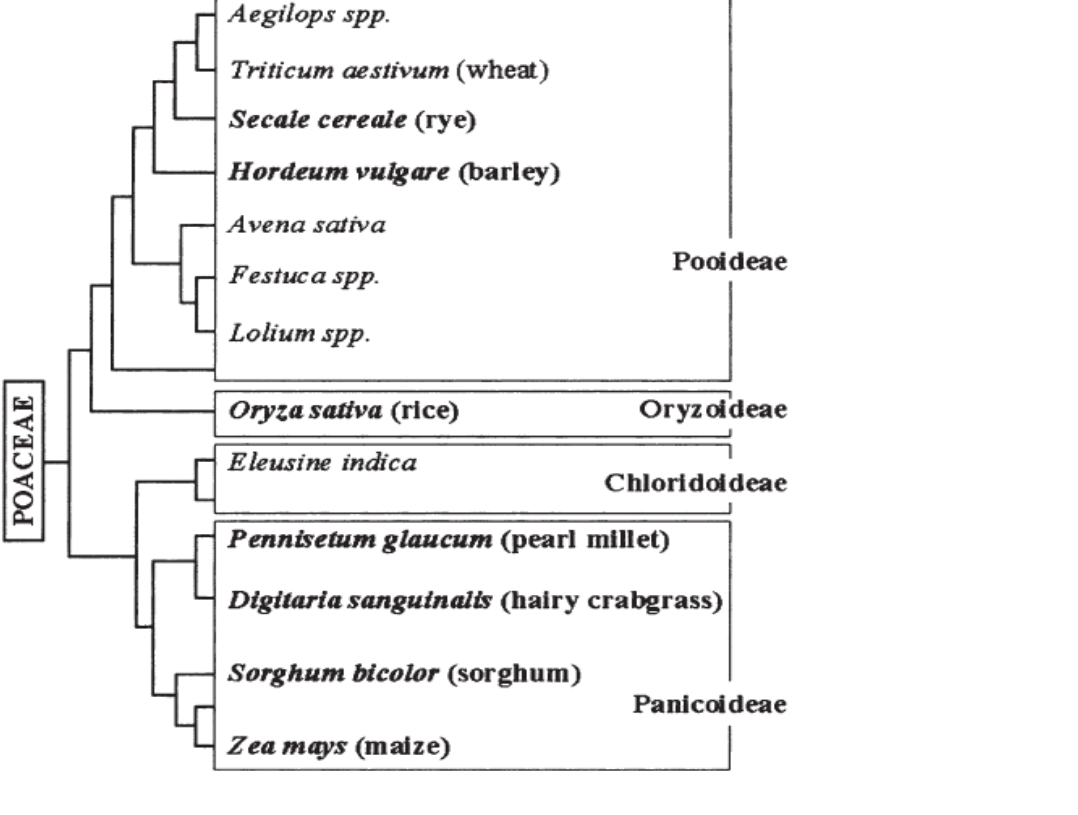
\includegraphics[width=10cm]{images/PoaceaePhylogeny}
  \end{center}
  \caption{Classification phylogénétique des Poacées \protect\cite{Paquet_2005}.}
  \label{fig:phylogenie_poacees}
\end{figure}


\subsection{Écologie}

\subsubsection{Photosensibilité}

Le sorgho est une plante de jours courts qui réagit de diverses façons
à la photopériode. À des latitudes élevées, certains cultivars
tropicaux ne fleurissent pas ou ne produisent pas de graines. Aux
États-Unis, en Australie et en Inde, on a noté l'existence de
cultivars moyennement sensibles à quasiment insensibles à la
photopériode \cite{BARRO_KONDOMBO_2010}.

\subsubsection{Conditions écologiques}

\paragraph{Conditions thermiques} Le sorgho tolère des températures de
tous niveaux. En effet, la sélection a permis de créer des variétés
cultivables en zones tempérées. Là où il ne gèle pas, le sorgho
continue à pousser et à produire de nouvelles feuilles vertes tant que
l'humidité du sol persiste. Il stoppe sa croissance sous les
8\,\degree{}C et meurt lorsque la température passe sous les
3\,\degree{}C\footnote{https://jardinage.ooreka.fr/plante/voir/2001/sorgho}. Il
est largement cultivé dans les régions tempérées et sous les tropiques
jusqu'à 2\,300 m d'altitude. La température optimale est de 25 à
31\,\degree{}C, mais des températures aussi faibles que 21\,\degree{}C
n'ont pas d'incidence grave sur la croissance et le rendement. Mais si
la température nocturne tombe en dessous de 12 à 15\,\degree{}C au
cours de la période de floraison, cela peut entraîner la stérilité. Le
sorgho est sensible au gel, mais moins que le maïs, et de légères
gelées nocturnes pendant la période de maturation provoquent peu de
dégâts \cite{BARRO_KONDOMBO_2010}.

\paragraph{Conditions hydriques} Le sorgho est une plante des milieux
tropicaux chauds et semi-arides qui sont trop secs pour les maïs
modernes en général (il existe des maïs de zones sèches). Il est
particulièrement adapté à la sécheresse en raison d'un ensemble de
caractéristiques morphologiques et physiologiques, notamment un
système racinaire étendu, la pruine de ses feuilles qui limite ses
pertes en eau (fig.~\ref{fig-SchemaComposePage5}
p.~\pageref{fig-SchemaComposePage5}), et une aptitude à interrompre sa
croissance pendant les périodes de sécheresse et à la reprendre une
fois le stress disparu. Le sorgho est une plante monocotylédone de la
tribu des Andropogoneae. Toutes les espèces de cette tribu présentent
une photosynthèse en $\text{C}_4$. La photosynthèse en $\text{C}_4$ se
réalise chez de nombreuses graminées tropicales à savoir le maïs, la
canne à sucre, le mil, le sorgho poussant dans des conditions
désertiques ou sur des sols salés. Elle se traduit par un type de
fixation du gaz carbonique où une enzyme cytoplasmique
phospho-énolpyruvate carboxylase catalyse une réaction avec comme
accepteur de $\text{CO}_2$ le phosphoénolpyruvate (PEP) :
$PEP + \text{CO}_2 \longrightarrow \text{Oxaloacétate}$. On parle de
photosynthèse en $\text{C}_4$ puisque l'on aboutit à la formation de
molécules à quatre atomes de carbone, contre trois pour les plantes en
$\text{C}_3$ (certaines graminées). Le sorgho est une plante en
$\text{C}_4$, ce qui lui donne un avantage compétitif lorsqu'elle est
soumise à la sécheresse, à la chaleur et à un faible taux d'azote
($\text{N}_2$) ou de dioxyde de carbone ($\text{CO}_2$). Par exemple,
lorsqu'elle est cultivée dans un environnement chaud (30\,\degree{}C),
elle perd moins de molécules d'eau : les graminées en $\text{C}_3$
perdent environ 833 molécules d'eau par molécule de $\text{CO}_2$
fixée tandis que le sorgho en perd seulement 277
\cite{sage1998c4}. Ceci offre donc un avantage aux plantes en
$\text{C}_4$ (sorgho) dans les environnements arides (zone sahélienne
au Burkina Faso) \cite{sage1998c4}. Des précipitations de 500 à 800 mm
également réparties pendant la saison de production conviennent
généralement aux cultivars qui mûrissent en 3 à 4 mois. Le sorgho
tolère un certain niveau d'asphyxie racinaire et on peut le faire
pousser dans des zones à fortes précipitations
\cite{BARRO_KONDOMBO_2010}.


\paragraph{Conditions édaphiques}
Le sorgho est bien adapté aux vertisols lourds. En pédologie un
vertisol est un sol riche en argile du type 2/1 c'est-à-dire contenant
une couche d'oxyde d'aluminium enserrée par deux couches de tétraèdres
de
silice\footnote{\url{https://www.memoireonline.com/06/12/5956/Analyse-des-determinants-de-la-faible-productivite-du-mas-a-Agadjaligbo-dans-la-commune-de-Zogbo.html}}
que l'on trouve couramment dans les tropiques, où sa tolérance à
l'asphyxie racinaire est souvent nécessaire, mais les sols sableux
légers lui conviennent tout autant. C'est toutefois sur les limons et
les limons sableux que sa culture réussit le mieux. La fourchette de
pH du sol supportée par le sorgho est de 5.0 à 8.5, et il tolère
davantage la salinité que le maïs (6 à
7.5)\footnote{\url{http://www.bioactualites.ch/fileadmin/documents/bafr/production-vegetale/grandes-cultures/4.5.11-73_Mais.pdf}}. Il
est adapté aux sols pauvres et peut produire du grain sur des sols où
beaucoup d'autres cultures échoueraient \cite{BARRO_KONDOMBO_2010}.


\subsection{Morphologie et biologie} La plante du sorgho
(\emph{Sorghum bicolor}) comprend une tige principale accompagnée de
talles issues du développement de bourgeons adventifs sur le collet du
maître brin. La hauteur de la plante à maturité varie beaucoup (de
50\,cm à plus de 5\,m). En fonction des cultivars et de leur
situation, les feuilles ---\,alternes, longues, retombantes, vert
clair ou vert foncé\,--- portées par les tiges varient en nombre, de
quelques unités à plus de 30 (fig.~\ref{fig-SchemaComposePage5}
p.~\pageref{fig-SchemaComposePage5}, \citeNP{BARRO_KONDOMBO_2010}). Le
\emph{Sorghum bicolor} est principalement autogame, mais une
pollinisation croisée par le vent peut se produire dans certaines
conditions, à plus de 60\,\% selon le génotype, et en moyenne environ
6\,\% \cite{Ellstrand_1983,
  House85,Pedersen_1998,Schertz_1980}. Puisque l'espèce se reproduit à
la fois par autopollinisation et par pollinisation croisée, la plupart
des races locales de sorgho cultivées par les agriculteurs de
subsistance sont constituées de mélanges de lignées pures et de
lignées partiellement pures \cite{SINGH_1997}. Le degré d'allogamie
varie notamment en fonction du type de panicule du cultivar ;
généralement, la pollinisation croisée est plus élevée dans le cas des
sorghos herbeux à panicule lâche que dans celui des sorghos cultivés à
panicule compacte. Selon certaines estimations, le taux d'allogamie
chez le sorgho cultivé en plein champ varie de 5 à plus de 40\,\%
\cite{Barnaud_2008, DJE_2004, Doggett_1988,
  Ellstrand_1983,Schmidt_2006}.

Plusieurs espèces de pollinisateurs ont été observées consécutivement
visitant des fleurs de sorgho cultivé \cite{Immelman_2000,
  Schmidt_2006}. Lors de la collecte des insectes, des grains de
pollen de sorgho ont été trouvés sur chacun de ceux-ci. Cependant, il
n'a pas été déterminé si le déplacement des insectes occasionnait une
pollinisation croisée. D'autres études doivent être réalisées pour
déterminer l'importance de la pollinisation par les insectes chez le
\emph{Sorghum bicolor}. La floraison et la pollinisation du
\emph{Sorghum bicolor} sont décrites dans \citeA{House85},
\citeA{SINGH_1997} et \citeA{SRINIVASA_2013}. L'inflorescence commence
à se former 30 à 40 jours après la germination. Le sorgho cultivé
fleurit généralement 55 à 70 jours après la germination en climats
chauds, mais, selon le génotype, la plante peut fleurir 30 à 100 jours
après la germination. Le temps humide et frais peut retarder la
floraison. Les fleurs commencent à s'ouvrir deux jours après que
l'inflorescence a émergé de la gaine. Les épillets (subdivisions de
l'inflorescence qui comportent plusieurs fleurs) sessiles, situés au
sommet de l'inflorescence, sont les premiers à fleurir, puis la
floraison se poursuit vers le bas de l'inflorescence durant 4 ou 5
jours. Chaque panicule peut comprendre jusqu'à 6\,000 fleurons
\cite{QUINBYKARPER_1947}. La floraison ne survient pas au même moment
chez toutes les inflorescences dans un champ, de sorte que le pollen
est généralement présent durant 10 à 15 jours.

Le moment de la floraison varie en fonction du génotype et du climat,
mais celle-ci se produit généralement du milieu de la nuit au milieu
de la matinée et atteint son maximum vers le lever du soleil. Le
gonflement des lodicules facilite l'ouverture des fleurs. Lorsque les
stigmates deviennent visibles, le filet des étamines s'allonge, et les
anthères deviennent pendantes. Une fois que les anthères sont sèches,
le pore apical s'ouvre et le pollen est libéré. La majeure partie du
pollen d'une inflorescence fertilise les ovules de la même
inflorescence. La pollinisation croisée est possible lorsque le pollen
est transporté dans les airs. Le stigmate est pollinisé avant que les
anthères émergent des épillets. Les grains de pollen sont transportés
jusqu'au stigmate et germent. Un tube pollinique se forme, et le grain
de pollen divisé en deux noyaux descend dans le style pour aller
fertiliser l'ovule. Un noyau spermatique fertilise l'ovule et produit
un embryon $2n$, et l'autre noyau fusionne avec les noyaux polaires
pour produire un albumen $3n$. Après la pollinisation, les glumes se
referment, et les anthères et stigmates vides en dépassent
généralement. Certaines variétés à glumes longues sont cléistogames
(les fleurons ne s'ouvrent pas pour la fertilisation). Les stigmates
non fécondés demeurent réceptifs jusqu'à seize jours. Après la
fertilisation, la différenciation des organes se déroule sur environ
douze jours. Les graines passent par trois stades de développement
---\,laiteux, pâteux mou et pâteux dur\,--- et parviennent à maturité
en environ 30 jours.

\subsection{Intérêt et utilisation du sorgho}

\emph{Sorghum bicolor} (L.) Moench est une céréale importante,
particulièrement pour les zones chaudes à pluviométrie réduite de la
zone tropicale. Le sorgho occupe le cinquième rang des plus
importantes céréales dans le monde, qu'il s'agisse du volume de la
production ou des superficies cultivées \cite{FAOICRISAT_1997}. En
Afrique subsaharienne, le sorgho est la deuxième céréale en importance
après le maïs. Le Nigeria en est le premier producteur de la région
avec 7\,\% de la production mondiale \cite{FAO_1995}
(tableau~\ref{tab:USDA_global_sorgho_production}
p.~\pageref{tab:USDA_global_sorgho_production}). Le sorgho est la
principale céréale cultivée au Burkina Faso, avec plus d'un million et
demi
d'hectares\footnote{\url{https://www.cirad.fr/nos-recherches/resultats-de-recherche/2016/la-selection-participative-du-sorgho-au-burkina-faso-creer-de-nouvelles-varietes-avec-et-pour-les-paysans}}. C'est
la plus importante culture vivrière dans les régions tropicales
semi-arides d'Afrique. Selon \citeA{Dahlberg_2011}, le sorgho est
l'aliment de base de 500 millions de personnes dans plus de 30 pays de
la zone tropicale
semi-aride\footnote{\url{http://www.memoireonline.com/01/14/8569/m_Contribution--l-etude-des-contraintes-de-stockage-des-cereales-mil-mas-sorgho-en-zone-sud-s8.html}}.
Sa culture y est pratiquée partout en saison des pluies, là où les
précipitations sont supérieures à 400 à 500 mm. La superficie
consacrée à la culture du sorgho est passée de 1\,016\,275 ha en
2\,000 à 1\,619\,590 ha en 2007 \cite{FAO_2007} et couvrait en 2016
1,8 millions
d'hectares\footnote{\url{http://www.commodafrica.com/14-11-2016-la-production-de-sorgho-en-afrique-progresseraitr-de-23-en-20161}}.

Dans les régions tropicales, le sorgho est essentiellement cultivé
pour son grain, destiné d'abord à l'alimentation humaine. Le grain
peut être consommé entier ou décortiqué et réduit en poudre pour faire
de la bouillie, du couscous, des beignets ou du \emph{tô} (nom d'un
des plats locaux cuisiné sous forme de pâte dans plusieurs pays
d'Afrique subsaharienne dont le Burkina Faso). Le grain peut être
fermenté pour donner des boissons alcoolisées : de la bière
(\emph{dolo})\footnote{Le dolo est une bière ancestrale obtenue par la
  fermentation du sorgho rouge ou du mil germé et cuit dans
  l'eau. Elle tire son nom d'une ville du Burkina Faso qui est le
  chef-lieu du département du même nom, situé dans la province
  Bougouriba et dans la région Sud-Ouest.} ou du vin de
sorgho\footnote{\url{https://www.doc-developpement-durable.org/file/Agriculture/Memento-de-l-Agronome_CIRAD.pdf}}.

\begin{table}
  \begin{footnotesize}
    \begin{center}
      \begin{tabular}{ld{2.3}d{2.3}d{2.3}d{2.3}d{2.3}d{2.3}}
        \multirow{3}{*}{} & \multicolumn{2}{c}{\textbf{Superficies}} & \multicolumn{2}{c}{\textbf{Rendements}} & \multicolumn{2}{c}{\textbf{Production}} \\
                          & \multicolumn{2}{c}{(millions ha)} & \multicolumn{2}{c}{(tonnes/ha)} & \multicolumn{2}{c}{(mégatonnes)} \\
                          & \multicolumn{1}{c}{2015/16} & \multicolumn{1}{c}{2016/17} & \multicolumn{1}{c}{2015/16} & \multicolumn{1}{c}{2016/17} & \multicolumn{1}{c}{2015/16} & \multicolumn{1}{c}{2016/17} \\ \hline
        Nigeria        & 5,30  & 5,30 & 1,16  & 1,23  & 6,15  & 6,50 \\
        Burkina        & 1,80  & 1,80 & 0,80  & 1,06  & 1,44  & 1,90 \\
        Mali           & 1,30  & 1,30 & 1     & 1     & 1,30  & 1,30  \\
        Niger          & 3,50  & 3,50 & 0,55  & 0,37  & 1,92  & 1,30  \\
        Ghana          & 0,25  & 0,25 & 1,05  & 1,20  & 0,26  & 0,30  \\ \hline
        \textbf{Afrique de l'Ouest} & 12,15  & 12,15 & 0,912 & 0,972  & 11,07  & 11,3  \\ \hline
        Ethiopie       & 1,50  & 1,80 & 1,73  & 2,06  & 2,60  & 3,70  \\
        Soudan         & 8     & 8    & 0,30  & 0,69  & 2,39  & 5,50  \\
        Cameroun       & 0,80  & 0,80 & 1,73  & 2,06  & 2,60  & 3,70  \\
        Tanzanie       & 0,80  & 0,80 & 1,03  & 1     & 0,82  & 0,80  \\
        Egypte         & 0,14  & 0,14 & 5,36  & 5,36  & 0,75  & 0,75  \\
        Ouganda        & 0,35  & 0,35 & 0,91  & 0,91  & 0,32  & 0,32  \\
        Mozambique     & 0,30  & 0,30 & 0,72  & 0,67  & 0,22  & 0,20  \\
        Afrique du Sud & 0,05  & 0,07 & 1,51  & 2,50  & 0,07  & 0,18  \\ \hline
        Afrique        & 24,09 & 24,41 & 1,35 & 1,49  & 19,39 & 23,9 \\
        \textbf{Monde} & 42,54  & 42,49 & 1,41 & 1,51 & 60,16 & 64,20 \\ \hline
      \end{tabular}
      \caption{Situations africaines et mondiale de production du
        sorgho, selon l'USDA (\emph{United States Department of
          Agriculture}) avec la production réelle (2015-2016) et les
        estimations
        (2016-2017)\protect\footnote{\protect\url{http://www.commodafrica.com/14-11-2016-la-production-de-sorgho-en-afrique-progresserait-de-23-en-201617}}.}
      \label{tab:USDA_global_sorgho_production}
    \end{center}
  \end{footnotesize}
\end{table}

\footnotetext{\url{http://www.commodafrica.com/14-11-2016-la-production-de-sorgho-en-afrique-progresserait-de-23-en-201617}}

Les tiges de certains \emph{Sorghum bicolor} sont consommées en frais
comme la canne à sucre et les résidus de récolte, soit l'ensemble des
tiges sont employées pour la confection des nattes, dans la
construction des maisons (matériaux de construction pour réaliser des
palissades) et des enclos ou comme combustibles,les feuilles et
panicules égrenées, représentent pour l'agriculteur une importante
source de fourrage pour l'alimentation de son bétail
\cite{Chantereau_1991}. Les graines (entiers) sont fournies
directement aux volailles \cite{SaintClair_1989}. Les cendres servent
à la préparation de la potasse alimentaire. Certains sorghos à forte
coloration tannique servent dans la teinture du cuir. Les extraits de
composés phénoliques servent en cosmétique pour le bronzage
\cite{BARRO_KONDOMBO_2010}. Si dans les principales régions
productrices d'Afrique et d'Asie, plus de 70\,\% du sorgho sont
consommés par les habitants aux Amériques et en Océanie, par contre la
plus grande partie de la production sert à l'alimentation animale
\cite{BARRO_KONDOMBO_2010}. La culture a également une vocation
industrielle orientée sur la production de la pâte à papier ou la
production de
fuel\footnote{\url{http://www.memoireonline.com/01/16/9362/m_Etude-de-la-diversite-agro-morphologique-du-sorgho-et-identification-de-cultivars-tolerants-au-str11.html}}.


\section{Le niébé: \emph{Vigna unguiculata} (L.) Walp.}

\subsection{Origine et diffusion}

Le niébé, \emph{Vigna unguiculata} est une légumineuse annuelle dont
le centre d'origine était incertain avant les études de Faris
\cite{FARIS_1963,FARIS_1965}. \citeA{Piper_1913} avait initialement
attribué une double origine au niébé : l'Inde et l'Afrique. Faris
\citeyear{FARIS_1963,FARIS_1965} après des études qui se sont reposées
sur une description cytologique et morphologique des formes sauvages
et cultivées du niébé montre que l'Afrique de l'Ouest et plus
probablement le Nigeria est le centre d'origine du niébé. Sa diffusion
vers l'Asie, en parallèle avec celle du sorgho, date de 2300
av. J-C. Le niébé est introduit en Europe vers 300 av. J-C où il reste
une culture mineure dans la partie méridionale. Les Espagnols et les
Portugais l'exportent au \textsc{XVII}\ieme{} siècle vers le nouveau
monde. D'autres cultivars sont transportés directement de l'Afrique
vers l'Amérique latine avec le trafic des esclaves. Le niébé atteint
le Sud des États-Unis au début du \textsc{XIX}\ieme{} siècle
\cite{Sawadogo_2009}.

\subsection{Taxonomie}

Le niébé a été décrit par \citeA{LINNE_1763}, à partir
d'une forme cultivée provenant des Antilles, sous le nom de
\emph{Dolichos unguiculatus}, qui deviendra \emph{Vigna unguiculata}
\cite{Pasquet_1997}. \emph{Vigna unguiculata} inclut des formes
cultivées et des formes sauvages. Les formes cultivées se distinguent
des formes sauvages par des gousses indéhiscentes, des graines et des
gousses de tailles plus importantes \cite{Lush_1981}. Selon
\citeA{Vanderborght_2001}, les formes cultivées sont regroupées dans
la sous-espèce \emph{unguiculata}, laquelle est subdivisée en quatre
cultigroupes: le cultigroupe Unguiculata (anciennement \emph{Vigna
  sinensis} (L.) Savi ex Hassk.)  forme couramment cultivée et plus
importante en Afrique ; le cultigroupe Biflora (anciennement
\emph{Vigna unguiculata} subsp. cylindrica (L.) Verdcourt), à petites
gousses érigées, cultivé principalement en Asie ; le cultigroupe
Sesquipedalis (anciennement \emph{Vigna unguiculata}
var. Sesquipedalis (L.) Ohashi), à gousses très longues et pendantes ;
le cultigroupe Texfilis avec de longs pédoncules est présent en
Afrique de l'Ouest. Le niébé est une dicotylédone de l'ordre des
Fabales, de la famille des Fabaceae, de la sous famille Faboideae, de
la tribu Phaseoleae, de la sous tribu des Phaseolinae, du genre
\emph{Vigna} \cite{Verdcourt_1970, Marechal_1978}.

%% Figure 5 : Quelques variétés de niébé (graines et plantes) observées au Burkina Faso
\begin{figure}%
  \begin{center}
    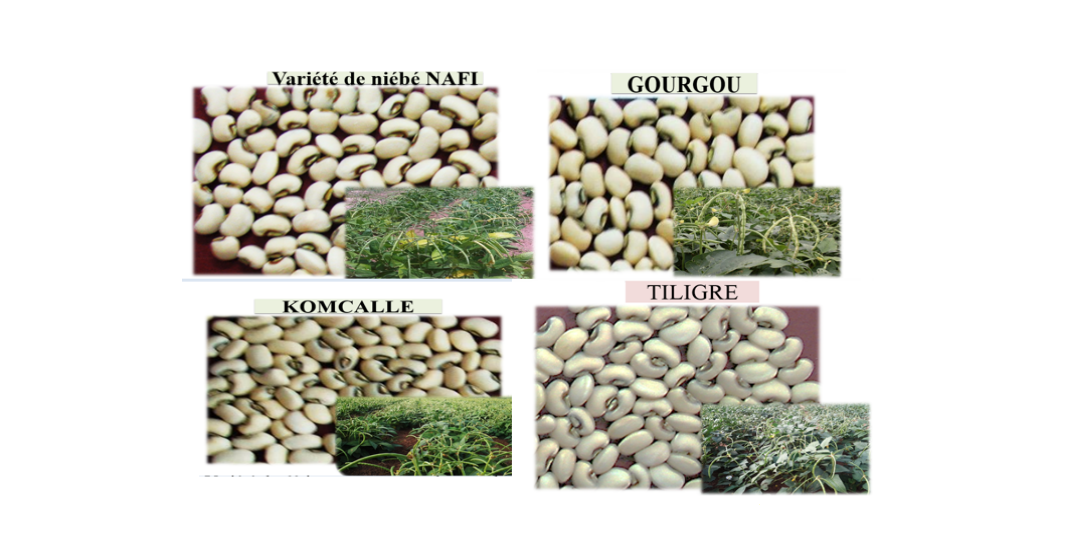
\includegraphics[width=12cm]{images/graines_niebe}
  \end{center}
  \caption{Quelques variétés de niébé observées au Burkina Faso}
\end{figure}

\subsection{Écologie}

\subsubsection{Photosensibilité}

Ce caractère a été largement étudié, en particulier par
\citeauthor{Steele_1972} \citeyear{Steele_1972}. On distingue trois
groupes, \textbf{le premier groupe}, photo-indépendant tardif,
comprend des génotypes indifférents à la photopériode
\cite{IITA_2008}. La croissance est indéterminée et le port
quelquefois érigé mais le plus souvent volubile. Ces génotypes sont
généralement tardifs et ont une floraison échelonnée à partir de nœuds
éloignés au cours de la saison culturale. On trouve ces cultivars dans
les zones les plus proches de l'équateur comme les savanes guinéennes
humides, où ils sont cultivés surtout en première saison
humide. \textbf{Le deuxième groupe}, photo-indépendant précoce, est
constitué des génotypes également indifférents à la photopériode. Ces
génotypes fleurissent précocement à partir des premiers nœuds de la
tige principale et donnent une production groupée, souvent récoltable
au bout de deux mois. Ces variétés sont cultivées dans les zones de
latitude élevée, en Inde, dans le bassin méditerranéen et aux
États-Unis. \textbf{Le troisième groupe}, photosensible, regroupe des
génotypes sensibles à la photopériode \cite{Steele_1972}. Le port est
généralement rampant et nettement moins volubile que chez les
cultivars du premier groupe. Ce groupe englobe la plupart des
cultivars traditionnels de la région soudano-sahélienne cultivés en
association avec le sorgho et le mil \cite{Doggett_1988}. Il est à
noter que les deux derniers groupes photo-indépendants précoce et
photosensible sont assez proches. Cultivés en jours très courts, ils
sont indiscernables et les cultivars photosensibles présentent alors
un port érigé et fleurissent dès les premiers nœuds. En revanche, les
deux premiers groupes photo-indépendant tardif et photo-indépendant
précoce sont bien distincts. Cultivés en jours longs, ils sont tardifs
mais leurs ports, rampant pour l'un et volubile pour l'autre,
apparaissent très différents. De plus, le groupe photo-indépendant
précoce et le groupe photosensible ont relativement peu d'ovules par
rapport au groupe photo-indépendant tardif. Ainsi, ce n'est pas le
photopériodisme qui permet de séparer les cultivars de niébé en deux
grands groupes physiologiques comme le supposait
\citeauthor{Steele_1972} \citeyear{Steele_1972}, mais l'aptitude à
fleurir rapidement dès les premiers nœuds de la tige principale dans
des conditions très inductives de jours courts \cite{IITA_2008}.

\subsubsection{Conditions édaphiques,thermiques,hydriques}

Le niébé se cultive sur les sols sableux à argileux. Il ne supporte
pas l'engorgement et l'acidité du sol \cite{Doggett_1988}. Le niébé
croît bien à des pH de 4,5 à 9,0 et réussit à fixer l'azote dans des
sols possédants moins de 2\,\% de matière organique et plus de 80\,\% de
sable \cite{SINGH_1997}. Le niébé est une culture très bien adaptée
aux régions arides et semi-arides. C'est une légumineuse cultivée
dans les régions tropicales et subtropicales \cite{Doggett_1988}. Le
niébé est une plante ayant une certaine adaptation à la
sécheresse. Sa culture est effectuée entre les isohyètes 300\,mm à
1\,500\,mm \cite{Doggett_1988}.

\subsection{Morphologie et biologie}


\paragraph{L'appareil végétatif} La \textbf{tige} du niébé est
cylindrique, volubile, quelques fois glabre et creuse. Elle définit le
port de la plante qui peut être érigé, semi-érigé, buissonnant, ou
rampant (fig.~\ref{fig:morphologie_niebe}). Chaque nœud de la tige
porte deux stipules et trois bourgeons axillaires. En ce qui concerne
les \textbf{feuilles}, la première paire est opposée et
monofoliée. Les secondes feuilles sont alternes et trifoliées
comprenant deux folioles opposées et une foliole terminale.Pour ce qui
est des \textbf{racines}, le système racinaire est pivotant avec de
nombreuses ramifications, ce qui confère au niébé une certaine
tolérance à la sécheresse. Les racines portent des nodosités de
bactéries fixatrices d'azote atmosphérique \cite{Doggett_1988}.

\paragraph{L'appareil reproducteur} L'\textbf{inflorescence} est un
racème axillaire. Le pédoncule a une longueur variable, au bout duquel
se trouve le rachis. La coloration des fleurs varie du blanc au violet
en fonction de la concentration d'anthocyanine. Le niébé est une
plante autogame \cite{Fery}. Le cycle des variétés est déterminé au
stade 50\,\% de floraison \cite{Drabo_1981}. Le \textbf{fruit} du
niébé est une gousse pendante ou dressée avec des formes linéaire,
spiralée, ou enroulée. La \textbf{gousse} peut être entièrement
pourpre, pigmentée sur les valves à son extrémité, marbrée ou
dépourvue de pigments. Les \textbf{graines} du niébé comporte un
tégument qui peut être ridé ou lisse. Elle est de couleur, de taille,
et de forme variables. La graine est riche en protéines et en
carbohydrates \cite{Doggett_1988}.

\begin{figure}%
  \begin{center}
    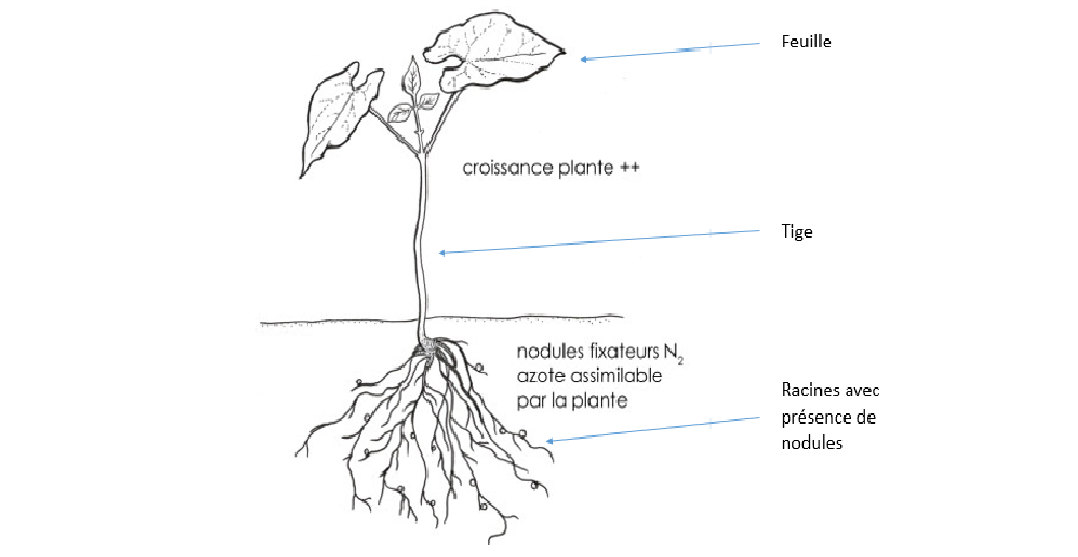
\includegraphics[width=14cm]{images/SchemaDescriptifNiebe}
  \end{center}
  \caption{Schéma illustrant la morphologie du
    niébé\protect\footnote{\protect\url{http://jardinonssolvivant.fr/WordPress/wp-content/uploads/2018/01/figure-1-1024x445.jpg}}.}
  \label{fig:morphologie_niebe}
\end{figure}

\footnotetext{\url{http://jardinonssolvivant.fr/WordPress/wp-content/uploads/2018/01/figure-1-1024x445.jpg}}

\subsection{Intérêt et utilisation du niébé}

Le terme niébé est un mot wolof désignant une plante légumineuse,
\emph{Vigna unguiculata} (L.) Walp. Herbacée africaine, sa culture
présente des retombées économiques, nutritionnelles et agronomiques
considérables entre autre dans de nombreux pays d'Afrique de l'Ouest y
compris les pays sahéliens tels que Burkina Faso où dans toutes les
régions du pays le niébé est produit avec une prédominance dans les
zones centre-nord et nord qui en sont de fortes productrices. La
campagne 2016/2017 du niébé montre que la culture  du niébé a occupée
228\,542 ha \cite{DGESS_2017}. Le
niébé est une source de devises pour les pays producteurs. Les graines
du niébé alimentent les échanges économiques au niveau régional et
sous régional. Selon \citeA{Langyintuo_2003} le Niger, le Burkina
Faso, le Bénin, le Mali, le Cameroun, le Tchad et le Sénégal sont les
principaux pays exportateurs du niébé ; tandis que le Nigeria, le
Ghana, le Togo, la Côte d'ivoire, le Gabon, et la Mauritanie sont les
pays importateurs. En plus du commerce des graines du niébé, le
fourrage est aussi commercialisé et utilisé dans l'alimentation des
animaux \cite{Langyintuo_2003}. En Afrique occidentale et centrale, le
commerce du fourrage du niébé permet une augmentation de 25\,\% du
revenu annuel des paysans \cite{Quin_1997}. Sur le plan nutritionnel:
les jeunes feuilles, les gousses immatures, et les graines sont
utilisées dans l'alimentation humaine. La valeur nutritionnelle des
graines est élevée avec en moyenne 23 à 25\,\% de protéines et 50 à
67\,\% d'amidon, ce qui confère au niébé un rôle important dans la
lutte contre la déficience protéique chez les enfants
\cite{Quin_1997}. Source de protéines moins coûteuse que celle
d'origine animale (viande, poisson, œufs), le niébé peut contribuer de
manière significative à la solution du problème de déficit protéique
souvent constaté en Afrique. De plus, les fanes de niébé sont un
aliment apprécié des animaux domestiques \cite{BAMBARA_2008}. La
graine du niébé est riche en lysine mais déficiente en acide aminé
soufré. Sur le plan agronomique, la culture du niébé permet un
enrichissement du sol en azote par l'intermédiaire de bactéries
fixatrices d'azote atmosphérique
(Rhizobiums\,\emph{s.l}). \citeA{Quin_1997}, montre qu'un hectare de niébé
fixe 40 à 80 kg d'azote nitrés dans le sol. De par sa croissance
rapide, le niébé assure une couverture du sol, le protégeant ainsi
contre l'érosion et contre l'envahissement par des adventices
\cite{Sawadogo_2009}.

\section{Les sols en Afrique subsaharienne: focus sur le Burkina Faso}

Le sol constitue le réservoir où les plantes puisent l'eau et les
éléments minéraux nécessaires à leurs besoins. La capacité de ce
réservoir dépend non seulement des caractéristiques du sol, mais aussi
de la profondeur exploitable par les racine. La texture et surtout la
structure du sol jouent un rôle important dans la dynamique de
l'enracinement des cultures \cite{Chopart_1980}. La structure
détermine aussi la masse volumique sèche (densité apparente) du sol et
par conséquent la porosité. Les propriétés physiques du sol
déterminent également ses caractéristiques hydrodynamiques, notamment
la perméabilité, la capacité au champ, le point de flétrissement
permanent et la réserve en eau utile
\footnote{\url{http://hydrologie.org/redbooks/a199/iahs_199_0217.pdf}}.


\begin{figure}%
  \begin{center}
    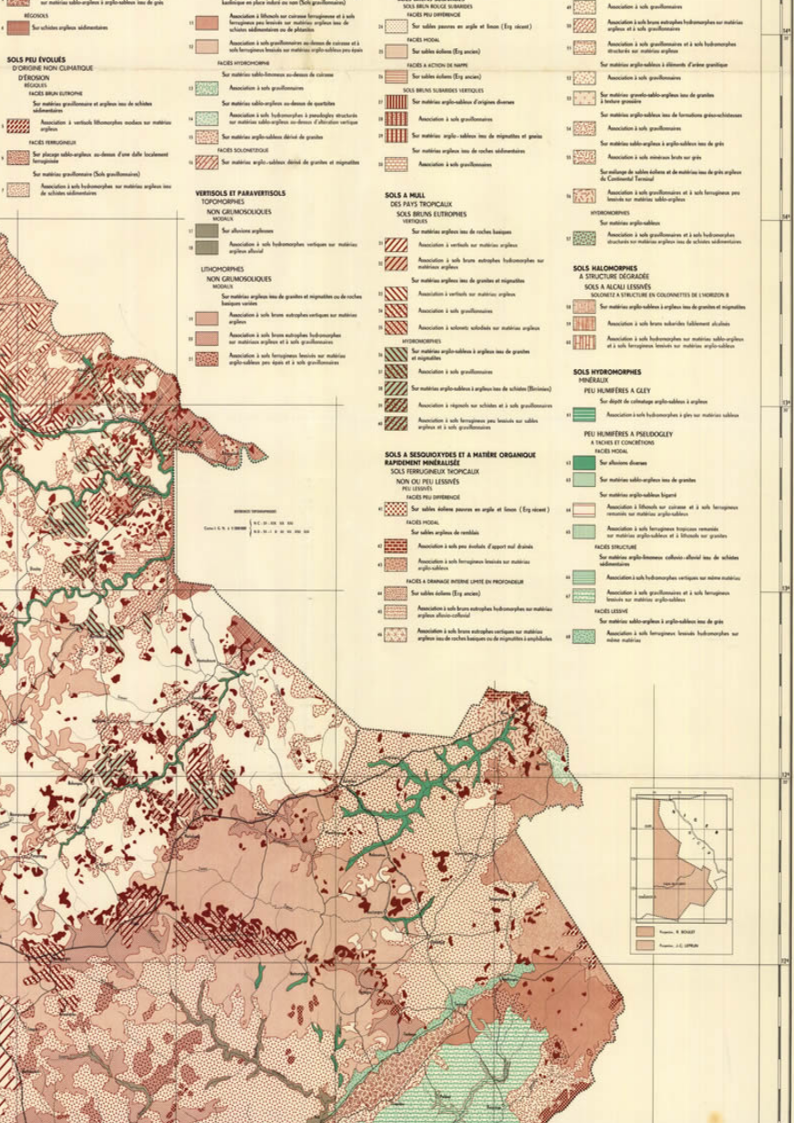
\includegraphics[width=12cm]{images/cartepedobf}
  \end{center}
  \caption{Carte des sols du Burkina Faso\,\protect\footnote{\protect\url{https://esdac.jrc.ec.europa.eu/ESDB_Archive/EuDASM/Africa/maps/afr_cpr_ha(es).htm}}.}
  \label{fig:carte_sols_burkina}
\end{figure}

\footnotetext{\url{https://esdac.jrc.ec.europa.eu/ESDB_Archive/EuDASM/Africa/maps/afr_cpr_ha(es).htm}}

Les sols du Burkina ont été étudiés par plusieurs institutions de
recherche et organismes de développement. En 1969, l'ORSTOM avait
réalisé une première couverture du territoire et dressé une carte
pédologique qui constitue toujours aujourd'hui la base de la plupart
des études pédologiques menées dans le pays
(fig.~\ref{fig:carte_sols_burkina}) \cite{BUNASOLS_1985}.  Les
pédologues ont classé l'ensemble des sols du pays en huit groupes
principaux proposés par le Bureau National des Sols (Bunasols) en 1985
sur la base d'autres études antérieures \cite{PERON_1975}. De façon
générale, les sols du Burkina ont un faible niveau de teneur en
éléments fertilisants, notamment en phosphore et en azote. Leur
profondeur est généralement limitée par une cuirasse qui affleure même
en surface en certains endroits. Le niveau de la réserve en eau varie
avec la toposéquence. Généralement faible en haut de pente (inférieure
à 60 mm/mètre de sol), la réserve utile peut dépasser 150 mm/mètre
dans les sols alluvionnaires le long des cours d'eau. C'est le cas par
exemple des sols de la plaine irriguée du Sourou
\cite{SOMENICOU_1983}. Ces sols subissent de façon très accrue le
ruissellement et l'érosion hydrique \cite{Roose_2004}. Il s'agit des
sols ferrugineux lessivés, des sols peu évolués d'érosion, des sols
bruns eutrophes, des vertisols, des sols ferrallitiques, des sols
halomorphes, des sols hydromorphes et des sols minéraux bruts avec une
dominance des sols ferrugineux dans la partie méridionale de la
pénéplaine précambrienne, au sud du 13\ieme\, parallèle. Ce sont des
sols à texture variable, généralement à tendance sableuse dans les
horizons de surface et argileuse dans les horizons plus profonds
(au-delà de 40\,cm). Ils ont un régime hydrique imparfait, en rapport
avec de mauvaises propriétés physiques (porosité et perméabilité). Ils
ont tous une faible capacité d'échange cationique. Ils sont
régulièrement associés à des sols gravillonnaires. Les sols peu
évolués d'érosion sont plutôt situés dans la moitié nord du pays. Ils
sont installés sur des granites et des migmatites dont ils
dérivent. Ils présentent un horizon sableux en surface (15 à 20\,cm)
et un horizon argileux au-delà. La compacité et l'imperméabilité de ce
second horizon jouent un rôle néfaste pour l'alimentation hydrique et
l'enracinement. Les sols hydromorphes sont installés sur des alluvions
fluviatiles ou sur des matériaux d'altération fins. De faible
drainage, ils s'engorgent régulièrement en saison des pluies. Ils sont
surtout développés dans l'ouest du pays et s'alignent avec le réseau
hydrographique majeur: vallées du Mouhoun, du Nazinon et du
Nakambé. Les sols bruns eutrophes sont caractérisés par une fraction
argileuse importante. La présence d'argile gonflante leur confère une
forte capacité d'échange et un taux de saturation élevé. Ce sont des
sols généralement bien drainés. Leur structure de surface est
variable, de grumeleuse à prismatique. C'est cette propriété qui règle
leur fertilité. Ils sont répartis sur l'ensemble du territoire, par
tâches de faible étendue. Les vertisols possèdent la même parenté
texturale que les sols bruns. De fait, ce sont des sols beaucoup moins
drainés. Ils sont particulièrement développés dans le sud-est et le
centre-ouest (vallée du Sourou). Les sols minéraux bruts sont des sols
de faible profondeur installés sur la roche-mère ou sur des horizons
cuirassés. Ce sont des sols pauvres. La végétation qu'ils portent est
tantôt clairsemée ou au contraire dense à cause de leur faible
aptitude agricole qui les met à l'abri de toute intervention
humaine. Les sols halomorphes ou salés sont installés au nord du
pays. De texture variée, ces sols ont une structure franchement
dégradée. Ce sont des sols pauvres qui supportent des steppes
arbustives extrêmement lâches. Les sols ferrallitiques sont localisés
dans le sud-ouest du pays où ils occupent une faible surface. Leur
profil s'apparente à celui des sols ferrugineux, mais leurs propriétés
physiques et chimiques les différencient nettement. Ils constituent de
bons supports pour les cultures et pour la végétation naturelle
dominée par les savanes arborées. Les sols de notre échantillonnage
ont été collectés sur des parcelles situées dans la zone
soudano-sahélienne du Burkina-faso (Boussouma, Kaya, Korsimoro). Trois
types de sols parmi ceux sus-cités sont rencontrés dans cette zone
d'étude: les sols ferrugineux tropicaux lessivés, les sols
hydromorphes peu humifères et les sols peu évolués d'érosion ou sols
sur cuirasse ferrugineuse \cite{TIROGO_2017}.

\section{Point sur la situation générale de la dégradation des sols au Burkina Faso}

Pays sahélien, le Burkina Faso est soumis depuis plusieurs décennies à
une forte dégradation de ses ressources naturelles, limitant ainsi le
développement des productions agro-sylvopastorales
\cite{Thiombiano_2000}. Cela est en relation avec le fait que le pays
connaitrait en général des conditions climatiques précaires, une
croissance démographique relativement élevée et une baisse continue de
la fertilité des sols. Les sols étant soumis à d'énormes contraintes
climatiques (érosions hydrique et éolienne, amplitudes thermiques,
etc.), deviennent très sensibles à la dégradation et ne supportent
pas, de façon soutenue, les systèmes et modes de production agricole
actuellement pratiqués \cite{PANA_2003}. À titre d'illustration, une
étude de \citeauthor{INERA_2003} montre que la dégradation affecte de
nos jours plus de 24\,\% des terres arables au Burkina
\cite{INERA_2003}, ce qui est préjudiciable à l'économie
nationale. Une autre étude plus récente estime également qu'environ
11\,\% des terres du pays sont considérées comme très dégradées et
34\,\%, comme moyennement dégradées \cite{SPCONEDD_2006}.  Les sols du
Burkina Faso sont naturellement pauvres en matières organiques
notamment en éléments nutritifs essentiels dont l'azote (N) et le
phosphore (P) \cite{Traore_2008} et ont une faible résistance à
l'érosion \cite{Berger_1991}. Aussi, les pays sahéliens en général et
le Burkina en particulier sont sensibles, vulnérables et en proie à
une diminution accélérée des ressources naturelles et à une
aggravation de la pauvreté dans les zones rurales
\cite{Roose_2004}. Les aspects les plus ressentis par les populations
restent la réduction significative de la couverture végétale avec une
crise du bois. Au Burkina Faso, étant donné que moins de 10\,\% de la
population a accès à d'autres sources d'énergie que le bois de feu,
près de 250\,000 hectares de forêts sont défrichés annuellement pour
satisfaire les besoins en bois de chauffe et 75\,000 hectares
supplémentaires sont convertis en nouveaux champs. Cette tendance est
toujours à l'augmentation. Dans le même temps, seuls 1\,000 hectares
sont
reboisés\footnote{\url{http://www.jle.com/fr/revues/sec/e-docs/bois_de_feu_et_deboisement_au_sahel_mise_au_point_265802/article.phtml}}. À
titre illustratif, les Mossis, sur les plateaux du Burkina Faso,
brûlent les pailles du mil, faute de bois, et appauvrissent leurs sols
déjà épuisés. Les rendements s'en ressentent, et la solution à court
terme consistant à écourter les périodes de jachère ne pouvant ainsi
avoir que des conséquences catastrophiques à long
terme\footnote{\url{http://archives-fig-st-die.cndp.fr/actes/actes_2007/bret/article.htm}}.
En parallèle de cette crise du bois, s'ajoutent la dégradation des
sols avec la perte de potentialités d'où une chute des rendements
agricoles, et une diminution des ressources hydriques avec
l'assèchement et l'ensablement des cours d'eau \cite{ZOMBRE_2006}.

\section{Avantage des pratiques culturales d'associations et de rotations de légumineuses-céréales:}

Les associations ou rotations de cultures sont des stratégies qui
s'inscrivent bien dans le cadre de l'intensification écologique
puisqu'elles visent à améliorer la productivité par unité de surface
cultivée sans recours à des intrants supplémentaires. Ce sont des
systèmes bien adaptés à la petite agriculture familiale, car ils
peuvent permettre de mieux protéger les sols, d'en améliorer la
fertilité à travers notamment la fixation symbiotique de l'azote par
les légumineuses, de faciliter le contrôle des mauvaises herbes. Les
associations de culture sont aussi une stratégie de minimisation des
risques pour des exploitations soumises à des températures élevées et
des précipitations faibles et souvent fluctuantes. Optimiser le
fonctionnement de ces systèmes qui sont déjà largement utilisés par
les paysans est donc un enjeu fort de recherche \& développement.


\subsection{Avantages et intérêts généraux}

\paragraph{Associations culturales} Les deux raisons les plus souvent
avancées pour l'adoption des associations d'espèces résident dans le
gain de rendement global par rapport à des cultures pures (mono
spécifiques) et dans l'amélioration significative et quasi
systématique de la teneur en protéines de la céréale, ceci quelle que
soit sa proportion dans le mélange récolté \cite{Jensen_1996}. Les
associations légumineuse-céréale permettent aussi une meilleure
valorisation des ressources du milieu comparativement aux cultures
mono-spécifiques correspondantes dans les systèmes à bas niveaux
d'intrants azotés \cite{Bedoussac_2010}. Les associations sont
également un moyen de réduire, dans certaines situations, la pression
des adventices, maladies et ravageurs \cite{Altieri_1999}, souvent
considérés comme des facteurs déterminants de la production agricole,
faisant ainsi des associations une alternative positive à la lutte
chimique \cite{Hauggaard_2001}.

Les mélanges d'espèces présentent aussi d'autres avantages comme : i)
la réduction de l'érosion des sols par une meilleure couverture et
enracinement \cite{Zougmore_1998}; ii) l'amélioration de la résistance
à la verse qui est un accident de végétation atteignant principalement
les céréales, provoqué par la pluie, le vent ou une attaque de
parasites et couchant les tiges au sol \cite{Anil_1998}; iii) la
réduction des risques de lixiviation qui traduit la perte de
nutriments végétaux hydrosolubles du sol (nitrates), qui sont dissous
et entraînés par les eaux de pluie ou d'irrigation
\cite{CorreHellou_2005} ou encore; iv) la meilleure stabilité
inter-annuelle des rendements \cite{Lithourgidis_2006}. En outre,
\citeauthor{Chu_2004} \citeyear{Chu_2004} ont aussi montré que le
système de culture intercalaire est très prometteur pour le
développement de la production alimentaire durable dans les conditions
de ressources naturelles limitées, et en particulier dans les
situations de ressources limitées en eau \cite{Tsubo_2005}. Dans le
cas spécifique d'association du niébé avec le sorgho, la plante du
sorgho aide celle du niébé à se développer
(fig.~\ref{fig:association_culturale}). De ce fait, les associations
culturales pourraient présenter un intérêt aussi bien en agriculture
biologique qu'en agriculture conventionnelle pour: i) améliorer la
qualité des composantes; ii) réduire les intrants chimiques; iii) et
améliorer les performances économiques et environnementales des
systèmes de production \cite{Koulibi_FideleZONGO}.

\begin{figure}
  \begin{center}
    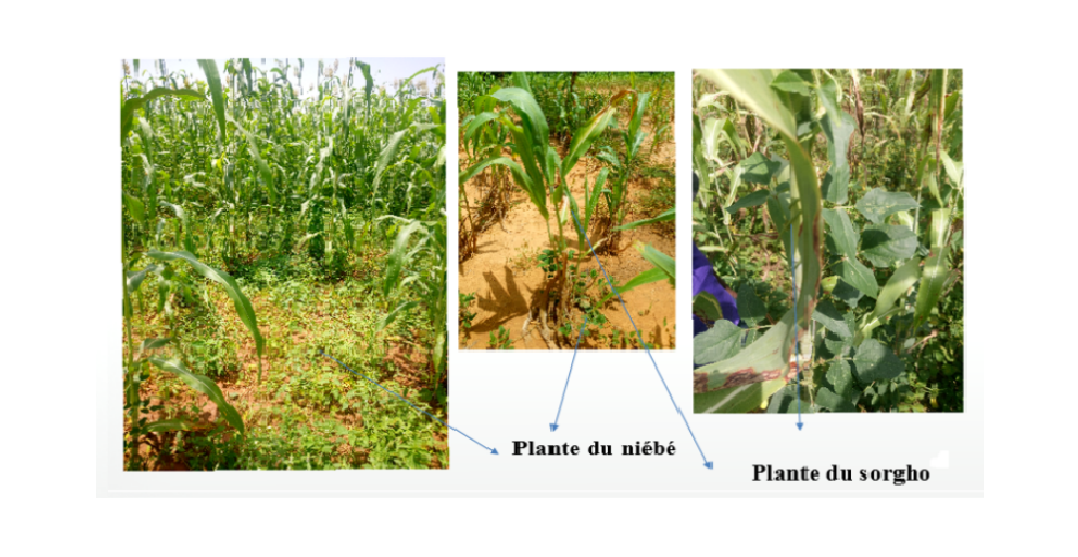
\includegraphics[width=16cm]{images/AssociationChampReel}
  \end{center}
  \caption{Représentation de l'association culturale en champ réel}
  \label{fig:association_culturale}
\end{figure}

\paragraph{Rotations culturales} Les rotations de culture consistent à
cultiver deux espèces avec un intervalle de temps donné. Il s'agit de
faire une suite de cultures échelonnées au fil des années sur une même
parcelle. En effet, le maintien et l'amélioration de la fertilité des
sols exigent l'utilisation des engrais organiques et
minéraux. Cependant les moyens économiques des paysans ne permettent
pas des interventions reposant sur des investissements importants. Il
devient alors nécessaire de mettre en œuvre des moyens naturels de
gestion de la fertilité des sols, comme la fixation biologique de
l'azote atmosphérique par les légumineuses dans un système de rotation
des cultures \cite{TRAORE_2009}. Les rotations de cultures constituent
un élément important de la gestion de la fertilité des sols et des
bioagresseurs, et donc représentent un atout pour l'augmentation des
rendements.


\subsection{Biodisponibilité de l'azote dans le sol}

Par leur capacité à fixer l'azote atmosphérique grâce au processus de
la fixation symbiotique, les légumineuses améliorent le bilan de
l'azote dans les systèmes de cultures
\cite{Ndakidemi_2005,Fustec11}. Lors de la fixation d'azote
atmosphérique, les légumineuses contribuent à la teneur en azote (N)
du sol sous forme organique ou
minérale\footnote{\url{http://fertilisation-edu.fr/cycles-bio-geo-chimiques/le-cycle-de-l-azote-n.html}}
(nitrates) soit en tant que cultures pures en rotation ou, en
association \cite{Bado_2006,Chu_2004,Makoi_2009,Ndakidemi_2005}. En
culture associée par exemple, les légumineuses peuvent augmenter la
teneur en azote du sol grâce à la fixation et l'excrétion
\cite{Trenbath_1976,Fustec11}. De ce fait, les plantes compagnes
bénéficient de la fixation biologique par les légumineuses et le
transfert ultérieur de l'azote des légumineuses aux
non-légumineuses. Plusieurs travaux scientifiques ont signalé que le
transfert de l'azote fixé par les légumineuses symbiotiques à la
céréale se fait par l'intermédiaire de la décomposition et de la
minéralisation des racines des légumineuses et/ou des nodules
\cite{Burity_1989} et par les exsudats racinaires libérés des
légumineuses \cite{Ndakidemi_2005,Makoi_2009}. Ce processus est appelé
rhizodéposition \cite{Fustec11} et constitue une source potentielle
d'accumulation de l'azote dans le sol \cite{Koulibi_FideleZONGO}. Le
niébé est une espèce généralement efficace dans la fixation de l'azote
grâce aux bactéries associées à ses racines \cite{TRAORE_2009}.

\newpage

\bibliographystyle{apacite}
\bibliography{revue_bibliographique}

\end{document}
